\chapter{Heuristics}
\label{chapAlgos}

\section{Linear Relaxation}

\subsection{General Relaxations}
\label{secAlgRelax}

Linear relaxation is a powerful and general technique for systematically obtaining an approximate solution to NP-Hard problems.
As was shown in Chapter \ref{chapHardness}, the RAAP is one such problem, so we look into this technique for approximating solutions.

In short, linear relaxation takes an Integer Linear Programme and removes the integrality constraints.
To understand how this works, we must consider the solution spaces of the various programmes, and it may help to think of these geometrically.
Let us suppose that the objective function for an ILP is a vector in high-dimensional space (one dimension for each variable), and the constraints are hyperplanes which form a convex polytope, called the feasible region.
If the solution could take arbitrary (real) values, then this is a (possibly unbounded) region, however, if the solution can only take integral values, then it is the set of integral coordinates in that region.
More formally, if $F$ is the $n$ dimensional polytope for real solutions, then $F \cap \mathbb{Z}^n$ are the feasible integral solutions.

This observation allows us to reason about the relative costs of the integral and linear solutions.
This difference is called the {\em integrality gap}, and is a well studied property of many NP-Hard problems, for example the integrality gap for the standard linear relaxation of Max-Cut is $2-\epsilon$ \cite{fer07}, where $\epsilon$ is some small ammount which depends on the number of constraints in the formulation.
When this gap is bounded, it provides a bound on the worst-case approximation so long as a relaxed linear programme is being used.

The next step in approximating is to round the real-valued solution to integer values.
This introduces a, possibly, larger margin and therefore increases the approximation ratio.
Rounding cannot typically be done in general (though there are general guidelines) and requires some structure from the specific problem to be used.
A clear example of this technique being used to solve a general processor assignment problem is presented by Lenstra, Shmoys and Tardos \cite{len87}.

\subsection{RAAP Relaxation}

For our specific problem we begin by relaxing our ILP formulation.
We repeat the integer programme from Section \ref{secModLin} here.
This programme currently solves the Robust Actor Assignment Problem to optimality.
To do this it must solve for the quadratic variable $\mathbf{Y}$ as explained in that section.
We remove the integrality constraints from this programme and treat it as a simple LP.

\begin{align}
	\nonumber \min & \sum_{a \in N; p \in P} \mathbf{I}_{a,p}\mathbf{X}_{a,p} + \sum_{a,b \in N; p,q \in P} \mathbf{C}_{a,b,p,q}\mathbf{Y}_{a,b,p,q} \\
	\nonumber s.t. &  \\
	\nonumber & \forall a \in N : \sum_{p \in P}\mathbf{X}_{a,p} = 1 \\
	\nonumber & \forall a,b \in N : \forall p,q \in P : \quad \mathbf{Y}_{a,b,p,q} \leq \mathbf{X}_{a,p} \\
	\nonumber & \forall a,b \in N : \forall p,q \in P : \quad \mathbf{Y}_{a,b,p,q} \leq \mathbf{X}_{b,q} \\
	\nonumber & \forall a,b \in N : \forall p,q \in P : \quad \mathbf{X}_{a,p} + \mathbf{X}_{b,q} - 1 \leq \mathbf{Y}_{a,b,p,q} \\
	\nonumber & \forall a,b \in N : \sum_{p \in P}\mathbf{Y}_{a,b,p,p}\mathbf{D}_{a,b} = 0
\end{align}

After obtaining a solution to the relaxed problem, we compute an integral solution via rounding.
To do this we must contrive a method of dealing with actors being assigned partially to multiple actors.
Fortunately the model ensures two things in this regard:
\begin{itemize}
	\item All actors are completely assigned (that is, the sum of all partial assignments is always 1).
	\item All parts of an actor's assignment reside on processors to which no parts of any of its replicas have been assigned.
\end{itemize}
\noindent We therefore will satisfy the non-overlapping constraint no matter which of the partial assignments we choose for the actor.
This allows us to assign actors greedily to whichever processor they are mostly already on, breaking ties arbitrarily.

\subsection{Issues with Relaxation}

As stated above, the approximation ratio is a function of the integrality gap and the rounding method.
We desire a fixed approximation ratio, and if possible a polynomial time approximation scheme which allows us to approximate, with the given ratio, the integral solution in polynomial time.
However, due to a difficulty which we elaborate on in this section, the discovery of such an approximation scheme is left as future work.

Recall Section \ref{secModLin} where we introduced a linearised version of quadratic terms in the first ILP formulation.
This step now warrants further examination.
Figure \ref{figAlgQuadratic} shows the quadratic curve $z=xy$ for $x$ and $y$ in the range $[0,1]$.
We relate this to the objective function for the integer programme shown in Section \ref{secModLin}, where $z$ means the tensor $\mathbf{Y}_{a,b,p,q}$ when $x$ means $\mathbf{X}_{a,p}$ and $y$ means $\mathbf{X}_{b,q}$. 
As we can see this curve can only be approximated with three dimensional planes and never fully realised.
More fundamentally this curve cannot be approximated at all by an unbounded convex polyhedron.

\begin{figure}
\begin{center}
	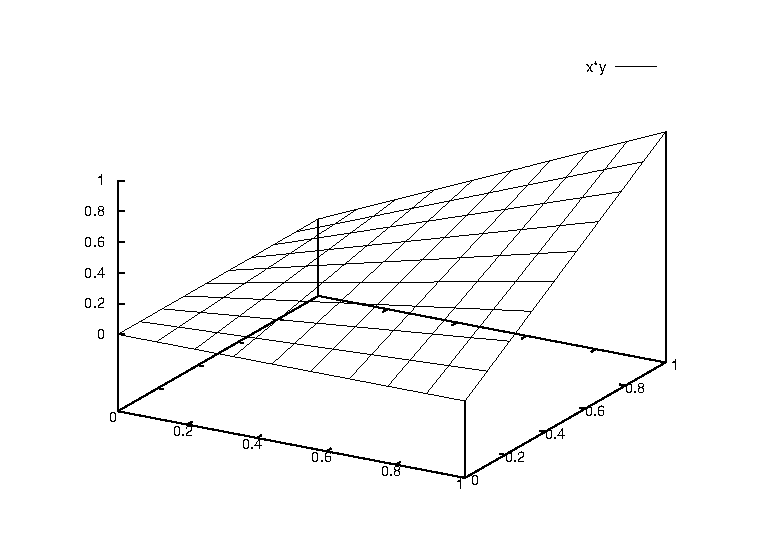
\includegraphics[width=12cm]{figures/quadratic.eps}
\caption{A quadratic curve for $x$ and $y$ in the range $[0,1]$}
\label{figAlgQuadratic}
\end{center}
\end{figure}

In the integral case $x$ and $y$ can only take the values $\{0,1\}$.
We are therefore able to capture this exactly using the linearised variable, and its three linearisation constraints.
Figure \ref{figAlgPlanes} shows the quadratic curve with the linearisation constraints overlayed (as planes).
As we see, these planes (along with the constraint that $z \geq 0$) force $z$ to take the correct values when $x$ and $y$ are integral.
However when the integrality constraints for $x$ and $y$ are dropped, the planes describe a much larger volume.
Though this volume contains the surface $z = xy$, given that the objective function is a minimisation one, the lower envelope of that volume does not accurately capture the surface.

\begin{figure}
\begin{center}
	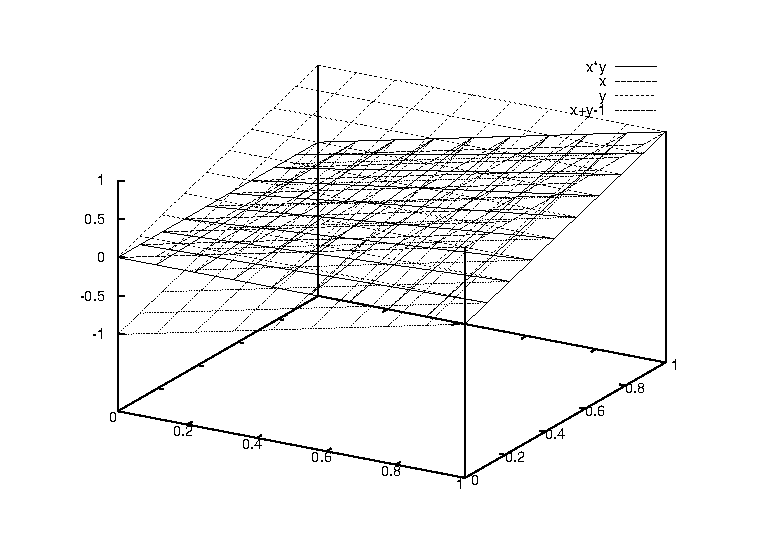
\includegraphics[width=12cm]{figures/approx.eps}
\caption{The quadratic curve from \ref{figAlgQuadratic} with the planes $z=x$, $z=y$ and $z=x+y-1$ overlayed}
\label{figAlgPlanes}
\end{center}
\end{figure}

This problem is the fundamental reason that using a relaxed linear solution to approximate the integral optimal is not possible.
Our ILP used the above hyperplanes to represent the quadratic surface, which only matches the actual surface at the integral points.
However where elements of the solution matrix $\mathbf{X}$ are assigned a non-integral value, the $\mathbf{Y}$ tensor will fail to represent the quadratic curve.
In other words, if the solver puts $0.4$ of actor $a$ on processor $p$, and $0.7$ of actor $b$ on processor $q$, then $\mathbf{Y}_{a,b,p,q}$ will take the value $\mathbf{X}_{a,p} + \mathbf{X}_{b,q} - 1 = 0.1$ instead of $\mathbf{X}_{a,p} \mathbf{X}_{b,q} = 0.28$.
This means that the ILP solver will be unable to correctly calculate the solution cost, and the solution is meaningless.

Indeed, the relaxed programme always gives a trivial zero-cost solution.
This is not an accurate calculation of the cost of the assignment, but it is correct as far as the LP is aware.
The solver simply assigns 0.5 of each actor to two available processors (provided there are enough).
Because the $\mathbf{Y}$ tensor does not accurately represent a quadratic curve, it takes a zero value wherever this happens.

This problem shows a fundamental weakness in the model, the integrality gap is unbounded.
The unbounded gap arises due to the linearisation of the quadratic term, which is only a correct representation where both it and the quadratic term have integral parameters.
The future work section (\ref{secConFut}) discusses the possibility of reformulating the problem to reduce the integrality gap.
An alternate formulation may attempt to have the solver working with the $\mathbf{Y}$ tensor outright, as opposed to deriving it from the $\mathbf{X}$ matrix.

\section{Heuristics}

\subsection{Motivation}

The linearisation of quadratic terms for the ILP solver also causes difficulties in running experiments.
It is well known that solving hard problems to optimality can take a long time for even small instances, however the linearisation makes this problem particularly acute, as the solver must deal with a large search space to find integral solutions.
For the RAAP, the brute force complexity is $O(p^n)$, where there are $n$ actors to assign to $p$ processors, when we exhaustively check each actor by allocating it to each processor.
The mathematical programme formulation must deal with the quadratic term, which has a large search space of $2^{np}$.
Smart use of branch-and-bound in the solver deals with this problem somewhat, still, on experimentation machines, the assignment of trivial SDF programs (12 actors, 4 processors) can take up to two hours.

The need for a faster means of assignment is therefore clear.
When dealing with problems of this nature the typical step is to use a known-worst-case approximation scheme which performs the task in polynomial time.
As the previous section mentioned, this step was unavailable to us, due again to the linearisation of quadratic constraints.

We therefore choose to implement a {\em heuristic} with unknown approximation ratio.
For this thesis we use the term heuristic to mean a feasible solution generator, where the solutions generated have unbounded costs in comparison to the optimal.
We distinguish this from an approximation scheme, such as relaxation and rounding techniques described in Section \ref{secAlgRelax}, where the solutions cost at worst better than some function of the optimal solution.
In practice heuristics are typically faster to run and simpler to implement than approximations.
This advantage comes at the cost of solution integrity, and some heuristics are known to perform arbitrarily badly in pathological cases.

Our heuristic is used to facilitate processor assignment for experiments.
Firstly we require the heuristic to even be able to run experiments on large instances ($> 100$ actors).
Large instances like this provide a more accurate impression of real-world SDF applications running on cloud systems, and hence it is valuable to not be limited to small testable instances.
Secondly we would like to examine the performance of the heuristic against optimal assignments.
Given that large instances take too long to assign optimally, this can only be done for relatively small graphs, however we should still be able to observe and generalise some properties of the heuristic in these tests.

\subsection{Algorithm}

The heuristic chosen is quite simple.
We note that certain elements can be optimised individually, even if the global optimal is not met, such as assigning actors individually to their best processor.
A greedy strategy can therefore be used to facilitate these assignments.
We know that we can determine the cost of any given assignment in polynomial time, so using a guess-and-check strategy for the greedy assignment will also be relatively quick.
That said the non-overlapping constraint is an important one which the heuristic must observe, though this does not prove to be much of a problem.

\begin{figure}
\begin{center}
	\fbox{
	\begin{minipage}{0.8\linewidth}
	\begin{algorithmic}
		\STATE $A$, set of actors
		\STATE $P$, set of processors
		\STATE $D_a \subseteq A$, set of duplicates for actor $a \in A$
		\STATE $\rSolution(a)$, mapping for actor $a$ ($\emptyset$ if $a$ is unassigned)
		\FORALL{$a \in A$}
			\STATE $P_a \leftarrow P \setminus \{\rSolution(b) | b \in D_a\}$
			\STATE $\rSolution' \leftarrow \rSolution$
			\FORALL{$p \in P_a$}
				\STATE $\beta \leftarrow \rSolution$
				\STATE $\beta(a) \leftarrow p$
				\IF{$\rSolution' = \rSolution$ or $\rCost(\rSolution') > \rCost(\beta)$}
					\STATE $\rSolution' \leftarrow \beta$
				\ENDIF
			\ENDFOR
			\STATE $\rSolution \leftarrow \rSolution'$
		\ENDFOR
		\STATE return $\rSolution$
	\end{algorithmic}
	\end{minipage}
	}
\caption{Processor Assignment Heuristic}
\label{figAlgAlg}
\end{center}
\end{figure}

The actual heuristic is shown in Figure \ref{figAlgAlg} as pseudocode.
As with the ILP itself, this algorithm can be used to assign graphs which do not have replication-type FT, this is done by simply presuming that no actors are duplicates.
This heuristic runs in time $O(np)$ when there are $n$ actors and $p$ processors.

Though simple, there is sufficient variability in the heuristic to allow for some interesting experiments.
For clarity, the above method assigns actor-duplicates individually, however it could be modified slightly so as to assign all duplicates of an actor at once.
More advantageously, the entire method could be iterated several times to improve the result.
This would allow actors, which were initially assigned without considering their communication costs, to be reassigned if it proves beneficial.
It is also much easier to modify this heuristic to evaluate the parallel makespan, rather than total costs.
This can be done by altering the cost function evaluated for each processor.

In general terms the heuristic is a greedy bin-packing algorithm.
It may also be useful to view the heuristic as a hill-climber, where it starts at some point in the feasible solution space and seeks a local maximum, though whether this is also a global maximum, or the heuristic even reaches it before terminating, is unknown.
It is sensitive to the order in which actors are evaluated, where initially assigning actors which are not directly connected to each other by an edge will skew the result to having a lower total invocation cost and much higher communication cost.
Chapter \ref{chapExperiment} will provide the experimental results on the performance of this heuristic when compared with the ILP's optimal solution.
